% article example for classicthesis.sty
\documentclass[10pt,a4paper]{article} % KOMA-Script article scrartcl
\usepackage{lipsum}
\usepackage{url}
\usepackage[nochapters]{classicthesis} % nochapters
\usepackage{polski}
\usepackage[utf8]{inputenc}
\usepackage{enumerate}
\usepackage{float}
\usepackage{subcaption}
\usepackage{graphicx}
\usepackage{amsmath}
\usepackage[T1]{fontenc}

\begin{document}
    \pagestyle{plain}
    \title{\rmfamily\normalfont\spacedallcaps{Opracowanie zagadnień na egzamin dyplomowy}}
    \date{} % no date

    \maketitle

    \tableofcontents

    \section{Zagadnienia obejmujące podstawowe treści programowe kierunku studiów Fizyka Techniczna do egzaminu dyplomowego na studiach II stopnia}
    \subsection{Ruch w mechanice newtonowskiej i relatywistycznej}
    
\begin{enumerate}[1]
\item \underline{Zasada dynamiki Newtona:}

I zasada dynamiki Newtona zakłada istnienie inercjalnego układu odniesienia. Układ inercjalny to taki, w którym cząstka nie podlegająca oddziaływaniu z otoczeniem, spoczywa lub porusza się po prostej ze stałą predkością (układy inercjalne poruszają się ruchem jednostajnym lub spoczywają względem siebie).

\item \underline{Zasada dynamiki Newtona:}
	
W inercjalnym układzie odniesienia jeśli siły działające na ciało nie rownoważą się ($ \vec{F_w} \neq 0 $) to ciało porusza się z przyśpieszeniem wprost proporcjonalnym do siły wypadkowej, a odwrotnie proporcjonalnym do masy ciała:\newline
$ \vec{a} = \frac{1}{m}*\vec{F_w} $\newline
$ \vec{F_w} = \frac{d\vec{p}}{dt} = \frac{d}{dt}(m\vec{v}) = m\frac{d\vec{v}}{dt} = m\vec{a} $\newline
Pierwsza zasada dynamiki Newtona jest szczególnym przypadkiem drugiej zasady dynamiki Newtona (gdy $ \vec{F_w} = 0 $).

\item \underline{Zasada dynamiki Newtona:}

Oddziaływania ciał są zawsze wzajemne. Jeżeli ciało \textit{A} działa na ciało \textit{B} siła $\vec{F}$ (akcja), to ciało \textit{B} działa na ciało \textit{A} siłą o takiej samej wartości i kierunku, lecz przeciwnym zwrocie (reakcja).
	
\end{enumerate}

\underline{Szczególna teoria względności}

\begin{enumerate}[1]
	\item \underline{postulat}:
	
We wszystkich układach inercjalnych prawa fizyki są jednakowe (zasada względności).

	\item \underline{postulat}:
	
Dla wszystkich obserwatorów inercjalnych prędkość światła w próżni (\textit{c}) jest taka sama i nie zależy od prędkości źródła światła.

\end{enumerate}

Te postualaty Einsteina prowadzą do tranformacji Lorentza:\newline
Rozważmy układ K oraz układ K' poruszający się względem K z predkością $ v_x $ wzdłuż osi OX (dla t = t' = 0 początki układów współrzednych $ 0_K $ i $ 0_{K'} $ pokrywają się), wtedy:\newline
$ t' = \gamma(\textit{t} - \frac{v_xx}{c^2}) $, $\gamma = \frac{1}{\sqrt{1-\frac{v_x^2}{c^2}}}$\newline
$ x'=\gamma(x - v_xt) $, y'=y, z'=z

Konsekwencje szczególnej teorii względności:

\begin{enumerate}[-]
\item Względność jednoczesności - dwa zdarzenia określone przez jednego obserwatora jako jednoczesne, mogą nie być jednoczesne dla innego obserwatora.
\item Dylatacja czasu - czas, jaki mija pomiędzy dwoma zdarzeniami, nie jest jednoznacznie określony, lecz zależy od ruchu obserwatora (paradoks bliźniąt).
\item Relatywistyczne składanie prędkości.
\item Masa jest równoważna energii $ E=mc^2 $.
\item Ciała bezmasowe poruszają się z prędkością c, dla ciał z niezerową masą niemożliwe jest osiągnięcie prędkości c.
\item Skrócenie Lorentza.
\end{enumerate}
    \subsection{Zasady zachowania i symetrie w fizyce}
	Jeśli układ posiada pewną symetrię, oznacza to, że równania opisujące ten układ nie zmieniają swojej postaci po dokonaniu przekształceń symetrii.

\underline{Dyskretne przekształcenia symetrii} to takie, których nie można sparametryzować np.
\begin{enumerate}[-]
	
\item Teoria grup i symetrii translacyjnej dla sieci periodycznej w kryształach.
\item Symetria permutacyjna funkcji falowej dla układu wielu ciał - związana z nierozróżnialnością cząstek elementarnych (zamiana miejscami cząstek układu nie zmiłaby równań opisujących układ).
\item Symetria zwierciadlana \textbf{P} związana z przekształceniem odbicia przestrzennego (zmiana znaków składowych przestrzennych wektorów na przeciwne).
\item Odwracalność w czasie \textbf{T} (zmiana znaku czasu w równaniach).
\item Parzystość ładunkowa \textbf{C} (zmiana znaku ładunku).

\end{enumerate}

Elektromagnetyzm, grawitacja i oddziaływania silne są niezmiennicze względem każdej z ostatnich trzech wymienionych symetrii (CPT) osobno, jednakże w przypadku oddziaływań słabych niezmienniczość jest zachowana tylko w przypadku łącznego ich działania CPT (rozpad $ \beta $ łamie symetrie P i C, ale zachowuje połączoną symetrie CP, która dla odmiany jest łamana w przypadku rozpadu mezonów K).

\underline{Symetrie związane z ciągłymi przekształceniami} są bezpośrednio związane z istnieniem zasad zachowania - związek ten opisuje twierdzenie Noether. Zgodnie z tym twierdzeniem, z daną symetrią układu jest związanych tyle praw zachowania, ile ciągłych rzeczywistych parametrów potrzebnych jest do sparametryzowania odpowiadających tej symetrii przekształceń np.

\begin{enumerate}[-]
\item Zasada zachowania energii wynika z symetrii związanej z przesunięciem w czasie - niezmienniczości działania S opisującego ruch danego układu od czasu (t - parametr). Jeżeli układ absorbuje lub emituje energie, wówcząs to działanie jest funkcją czasu (t) - odpowiada to w konsekwencji zmianie energii układu.

\item Zasada zachowania pędu wynika z symetrii związanej z przesunięciem układu w przestrzeni.

\item Zasada zachowania momentu pędu wynika z z symetrii związanej z obrotem układu.

\item Zasada zachowania ładunku wyniki z niezmienniczości funkcji falowej elektronu względem transformacji cechowania.
\end{enumerate}
	\subsection{Klasyczny i kwantowy oscylator harmoniczny}
	Lalala
	\subsection{Fizyczna treść równań Maxwella i równania falowego.}
	\begin{figure} [H]
	\centering
	\begin{subfigure}{.49\textwidth}
		\centering
		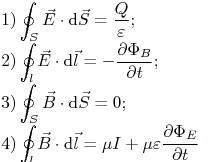
\includegraphics[width=1.0\linewidth]{generalIssues/Figures/maxwell1.png}
		\caption{Postać całkowa.}
		\label{n1}
	\end{subfigure}
	\begin{subfigure}{.49\textwidth}
		\centering
		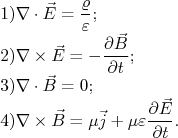
\includegraphics[width=1.0\linewidth]{generalIssues/Figures/maxwell2.png}
		\caption{Postać różniczkowa.}
		\label{r1}
	\end{subfigure}
	\caption{Równania Maxwella.}
	\label{maxwell}
\end{figure}

Rysunek~\ref{maxwell} przedstawia równania Maxwella, gdzie:\newline
$ \varrho $ - gęstość ładunku,\newline
$ \varepsilon $ - przenikalność dielektryczna,\newline
$ \mu $ - przenikalność magnetyczna,\newline
$ \vec{j} $ - gęstość prądu,\newline
$ \Phi_B $- strumień indukcji magnetycznej,\newline
$ \Phi_E $- strumień natężenia pola elektrycznego,\newline
$ \nabla * \vec{F} = \frac{\partial F_x(x,y,z)}{\partial x} + \frac{\partial F_y(x,y,z)}{\partial y} + \frac{\partial F_z(x,y,z)}{\partial z}$ - dywergencja pola wektorowego $ \vec{F} = [F_x, F_y, F_z] $,\newline
$
\nabla \times \vec{F} = 
\begin{vmatrix}
\textbf{i} & \textbf{j} & \textbf{k} \\ 
\frac{\partial}{\partial x} & \frac{\partial}{\partial y} & \frac{\partial}{\partial z} \\ 
F_x & F_y & F_z  \notag
\end{vmatrix}
= (\frac{\partial F_z}{\partial y} - \frac{\partial F_y}{\partial z})\textbf{i} + (\frac{\partial F_x}{\partial z} - \frac{\partial F_z}{\partial x})\textbf{j} + (\frac{\partial F_y}{\partial x} - \frac{\partial F_x}{\partial y})\textbf{k}
$ - rotacja pola wektorowego $ \vec{F} $.\newline

Sens fizyczny praw Maxwella:
\begin{enumerate}[1)]
	\item \underline{Prawo Gaussa dla elektryczności} - źródłem pola elektrycznego są ładunki, a strumień tego pola przez dowolną powierzchnię zamkniętą zależy tylko od ładunku zamkniętego przez tę powierzchnię.
	\item \underline{Prawo Faradaya} - zmiana strumienia indukcji magnetycznej przez powierzchnię zamkniętej pętli powoduje powstanie w tej pętli siły elektromotorycznej indukcji (SEM), a kierunek płynącego prądu jest taki, żeby przeciwdziałać zmianom powodującym indukcję (reguła Lenza).
	\item \underline{Prawo Gaussa dla magnetyzmu} - nie istnieją ładunki magnetyczne, a strumień pola magnetycznego przez dowolną powierzchnię zamkniętą jest równy 0.
	\item \underline{Prawo Ampere'a} - zmienne pole elektryczne i płynący prąd powodują powstanie pola magnetycznego.
\end{enumerate}

Dla fali elektromagnetycznej w próżni wektory $ \vec{E} $ i $ \vec{B} $ drgają w płaszczyznach wzajemnie prostopadłych i dla fali rozchodzącej się w kierunku osi x możemy przyjąć taki układ odniesienia aby wektor $ \vec{E} $ drgał w kierunku osi y a wektor $ \vec{B} $ w kierunku osi z. Zatem wektory $ \vec{E} $ i $ \vec{B} $ mają tylko po jednej składowej:\newline
$ \vec{E} = [0, E, 0] $,\newline
$ \vec{B} = [0, 0, B] $.\newline
Liczmy rotację wektorów $ \vec{E} $ i $ \vec{B} $ (wykorzystując fakt, że nasza fala jest falą płaską i pola $ \vec{E} $ i $ \vec{B} $ zmieniają się tylko względem współrzędnej x, czyli że $ \frac{\partial E}{\partial z} = 0, \frac{\partial B}{\partial y} = 0$):\newline
$ \nabla \times \vec{E} = \textbf{k}\frac{\partial E}{\partial x} $,\newline
$ \nabla \times \vec{B} = -\textbf{j}\frac{\partial B}{\partial x} $.\newline

Korzystając z równań Faradaya oraz Ampera w postaci różniczkowej otrzymujemy (poszukujemy równania dla fal elektromagnetycznych rozchodzących się w próżni gdzie nie będą występowały prądy przewodzenia, czyli $ \vec{j} $ = 0):\newline
$ \textbf{k}\frac{\partial E}{\partial x} = -\frac{\partial \vec{B}}{\partial t} = -\textbf{k}\frac{\partial B}{\partial t} $,\newline
$ \textbf{j}\frac{\partial B}{\partial x} = -\mu_0 \epsilon_0 \frac{\partial \vec{E}}{\partial t} = -\textbf{j} \mu_0 \epsilon_0 \frac{\partial E}{\partial t} $.\newline
W efekcie dostajemy układ dwóch równań:\newline
$ \frac{\partial E}{\partial x} = -\frac{\partial B}{\partial t} $,\newline
$ \frac{\partial B}{\partial x} = - \mu_0 \epsilon_0 \frac{\partial E}{\partial t} $.\newline

Równania falowe dla $ \vec{E} $ i $ \vec{B} $ będą miały identyczną postać. Jeżeli zdecydujemy się szukać równania dla $ \vec{E} $, to eliminujemy z naszego układu równań $ \vec{B} $ przez utworzenie pochodnych mieszanych $ \vec{E} $ względem x i t. Różniczkujemy zatem pierwsze równanie po x, a drugie po t (jeśli chcemy szukać równania dla $ \vec{B} $ eliminujemy w ten sam sposób z naszych równań $ \vec{E} $):\newline
$ \frac{\partial^2 E}{\partial x^2} = -\frac{\partial^2 B}{\partial t \partial x} $,\newline
$ \frac{\partial^2 B}{\partial t \partial x} = - \mu_0 \epsilon_0 \frac{\partial^2 E}{\partial t^2} $.\newline
Z powyższego układu równań otrzymujemy poszukiwane równanie falowe dla pola $ \vec{E} $:\newline
$ \frac{\partial^2 E}{\partial x^2} - \mu_0 \epsilon_0 \frac{\partial^2 E}{\partial t^2} = 0 $\newline
Znając ogólną postać równania falowego dla fali rozchodzącej się z predkością v w kierunku osi x:\newline
$ \frac{\partial^2 \xi}{\partial x^2} - \frac{1}{v^2} \frac{\partial^2 \xi}{\partial t^2} = 0 $\newline
otrzymujemy związek pomiędzy prędkością światła w próżni (c) a wartościami przenikalności elektrycznej i magnetycznej próżni: \newline
$ c = \frac{1}{\sqrt{\mu_0 \epsilon_0}} $.\newline
Rozwiązanie równania falowego dla pola $ \vec{E} $ ma postać:\newline
$ \vec{E} = \vec{E_0}\sin(kx - \omega t) $,\newline
gdzie: $ k = \frac{2\pi}{\lambda} $, $ \omega = ck $.
	
	\subsection{Właściwości fal elektromagnetycznych.}
	Falą elektromagnetyczną nazywamy rozchodzące się w przestrzeni zaburzenie pola elektromagnetycznego. Składowa elektryczna i magnetyczna fali indukują się wzajemnie – zmieniające się pole elektryczne wytwarza zmieniające się pole magnetyczne, a z kolei zmieniające się pole magnetyczne wytwarza zmienne pole elektryczne.

Promieniowanie elektromagnetyczne przejawia właściwości falowe ulegając interferencji, dyfrakcji, spełnia prawo odbicia i załamania. W wyniku superpozycji fal elektromagnetycznych może powstać fala stojąca. 

Strumień energii przenoszonej przez falę elektromagnetyczną w każdym punkcie przestrzeni określa wektor Poyntinga zdefiniowany jako:\newline
$ \vec{S} = \frac{1}{\mu_0} \vec{E} \times \vec{B} $,\newline
gdzie:\newline
$ \mu_0 $ - przenikalność magnetyczna próżni,\newline
$ \vec{E} $ - natężenie pola elektrycznego,\newline
$ \vec{B} $ - indukcja pola magnetycznego.

Choć w elektrodynamice klasycznej energię promieniowania elektromagnetycznego uważa się za wielkość ciągłą, zależną jedynie od natężenia pola elektrycznego i indukcji pola magnetycznego, to zjawiska zachodzące na poziomie atomowym dowodzą, że jest ona skwantowana. Energia pojedynczego kwantu jest zależna tylko od częstotliwości fali $ \nu $ i wynosi:\newline
$ E = h \nu $, gdzie \textit{h} - stała Plancka.

Właściwości fal elektromagnetycznych zależą od długości fali. Promieniowaniem elektromagnetycznym o różnej długości fali są:
 
\begin{enumerate}[-]
	\item \underline{Fale radiowe} (długość fali powyżej 1 m) - znajdują bardzo szerokie zastosowanie w telekomunikacji, radiofonii, telewizji, radioastronomii i wielu innych dziedzinach nauki i techniki. Naturalne źródła fal radiowych to między innymi wyładowania atmosferyczne, zorze polarne, radiogalaktyki.
	\item \underline{Mikrofale} (od 1 mm do 1 m) - podstawowe zastosowania mikrofal to łączność (na przykład telefonia komórkowa, radiolinie, bezprzewodowe sieci komputerowe) oraz technika radarowa. Fale zakresu mikrofalowego są również wykorzystywane w radioastronomii, a odkrycie mikrofalowego promieniowania tła miało ważne znaczenie dla rozwoju i weryfikacji modeli kosmologicznych. Wiele dielektryków mocno absorbuje mikrofale, co powoduje ich rozgrzewanie i jest wykorzystywane w kuchenkach mikrofalowych, przemysłowych urządzeniach grzejnych i w medycynie.
	\item \underline{Podczerwień} (od 700 nm do 1 mm) - promieniowanie podczerwone jest nazywane również cieplnym, szczególnie gdy jego źródłem są nagrzane ciała. Każde ciało o temperaturze większej od zera bezwzględnego emituje takie promieniowanie, a ciała o temperaturze pokojowej najwięcej promieniowania emitują w zakresie długości fali rzędu 10 $ \mu m $. Przedmioty o wyższej temperaturze emitują promieniowanie o większym natężeniu i mniejszej długości, co pozwala na zdalny pomiar ich temperatury i obserwację za pomocą urządzeń rejestrujących wysyłane promieniowanie (termowizja).
	\item \underline{Światło widzialne} (od 380 nm do 700 nm) - światło (promieniowanie widzialne) to ta część widma promieniowania elektromagnetycznego, na którą reaguje zmysł wzroku człowieka. Różne zwierzęta mogą widzieć w nieco różnych zakresach. Światło ma bardzo duże znaczenie w nauce i wiele zastosowań w technice. Dziedziny nauki i techniki zajmujące się światłem noszą nazwę optyki.
	\item \underline{Ultrafiolet} (od 10 nm do 380 nm) - promieniowanie ultrafioletowe jest zaliczane do promieniowania jonizującego, czyli ma zdolność odrywania elektronów od atomów i cząsteczek. W technice ultrafiolet stosowany jest powszechnie. Powoduje świecenie (fluorescencję) wielu substancji chemicznych. W świetlówkach ultrafiolet wytworzony na skutek wyładowania jarzeniowego pobudza luminofor do świecenia w zakresie widzialnym. Niektóre owady, na przykład pszczoły, widzą w bliskiej światłu widzialnemu części widma promieniowania ultrafioletowego, również rośliny posiadają receptory ultrafioletu. 
	\item \underline{Promieniowanie rentgenowskie} (od 5 pm do 10 nm) - promieniowanie rentgenowskie jest promieniowaniem jonizującym. Technicznie promieniowanie rentgenowskie uzyskuje się przeważnie poprzez wyhamowywanie rozpędzonych cząstek naładowanych. W lampach rentgenowskich są to rozpędzone za pomocą wysokiego napięcia elektrony hamowane na metalowych anodach. Źródłem wysokoenergetycznego promieniowania rentgenowskiego są również przyspieszane w akceleratorach cząstki naładowane. Promieniowanie rentgenowskie jest wykorzystywane do wykonywania zdjęć rentgenowskich do celów defektoskopii i diagnostyki medycznej. W zakresie promieniowania rentgenowskiego są również prowadzone obserwacje astronomiczne. 
	\item \underline{Promieniowanie gamma} (0,03 pm do 300 pm) - promieniowania gamma jest promieniowaniem jonizującym. Promieniowanie gamma towarzyszy reakcjom jądrowym, powstaje w wyniku anihilacji – zderzenie cząstki i antycząstki, oraz rozpadów cząstek elementarnych. Otrzymywane w cyklotronach promieniowanie hamowania i synchrotronowe również leży w zakresie długości fali promieniowania gamma, choć niekiedy bywa nazywane wysokoenergetycznym promieniowaniem rentgenowskim. Promienie gamma mogą służyć do sterylizacji żywności i sprzętu medycznego. W medycynie używa się ich w radioterapii oraz w diagnostyce. Zastosowanie w przemyśle obejmują badania defektoskopowe. Astronomia promieniowania gamma zajmuje się obserwacjami w tym zakresie długości fal. 
\end{enumerate}
	
	\subsection{Interferencja i dyfrakcja fal.}
	\underline{Interferencja} jest to zjawisko powstawania nowego, przestrzennego rozkładu amplitudy fali (wzmocnienia i wygaszenia) w wyniku nakładania się (superpozycji fal) dwóch lub więcej fal. Warunkiem trwałej interferencji fal jest ich spójność, czyli korelacja faz i równość częstotliwości. 

Dla najprostszego przypadku dwóch fal harmonicznych o jednakowych amplitudach A, jednakowej długości fali $ \lambda $ i zgodnych fazach początkowych, rozchodzących się z dwóch różnych źródeł, które leżą w odległościach odpowiednio $ d_1 $ i $ d_2 $ od punktu P, zaburzenie w punkcie P opisuje wzór:\newline
$ y(P) = A\sin (\omega t + \phi_1) + A\sin (\omega t + \phi_2)$, gdzie:\newline
$ \phi_1 = 2\pi\frac{d_1}{\lambda} $,\newline
$ \phi_2 = 2\pi\frac{d_2}{\lambda} $.\newline
Gdy spełniony jest warunek:\newline
$ \phi_1 - \phi_2 = 2\pi\frac{d_1-d_2}{\lambda} = 2k\pi $,\newline
gdzie k - dowolna liczba naturalna, to fale w punkcie P ulegają wzmocnieniu (są w tej samej fazie) i:\newline
$ y(P) = 2A\sin (\omega t) $.\newline
Gdy natomiast w pewnym punkcie $ P_1 $:\newline
$ \phi_1 - \phi_2 = 2\pi\frac{d_1-d_2}{\lambda} = (2k+1)\pi $\newline
wtedy fale wygaszają się (są w przeciwfazie) i:\newline
$ y(P_1) = 0 $.

Interferencja pozwala na bardzo precyzyjny pomiar zmian długości drogi od źródła do detektora fali.

\underline{Dyfrakcja} (ugięcie fali) – zespół zjawisk związanych ze zmianą kierunku rozchodzenia się fali będący odstępstwem od praw optyki geometrycznej (dział optyki zajmujący się wytłumaczeniem zjawisk optycznych przy użyciu pojęcia promienia). Dyfrakcję w węższym znaczeniu określa się jako ugięcie światła wokół krawędzi przeszkody lub otworu w obszarze cienia przeszkody.

Zjawisko dyfrakcji rozpatruje się jako interferencję fal cząstkowych powstających zgodnie z zasadą Huygensa. Jest to zasada stosowana do określenia rozchodzenia się fali w ośrodku, mówiąca, iż każdy punkt ośrodka, do którego dotarło czoło fali, można uważać za źródło nowej fali kulistej. Wypadkową powierzchnię falową tworzy powierzchnia styczna do wszystkich powierzchni fal cząstkowych i ją właśnie obserwuje się w ośrodku.

Rysunek~\ref{diffracion} przedstawia dyfrakcję na pojedynczej szczelinie. Gdy różnica dróg fali ze skrajnego i środkowego elementu równa jest połowie długości fali, to fale z obu połówek szczeliny wygaszą się. Jeżeli wiązki są niemal równoległe, to różnica odległości pojawia się tylko przy wyjściu promieni ze szczeliny, wówczas:\newline
$ d\sin(\theta_{min}) = \lambda $.\newline

Przepuszczenie fali przez szczelinę dyfrakcyjną pozwala na określenie kierunku rozchodzenia się fali. Im mniejsza jest szerokość szczeliny, tym dokładniej można to zrobić. Jednocześnie zmniejszanie szczeliny powoduje, że trudniej jest określić energię fali, ponieważ rozprasza się ona na większy obszar. W efekcie iloczyn błędu określenia energii oraz błędu pomiaru kierunku musi być większy od pewnej stałej. Oznacza to, że istnieje granica dokładności pomiaru parametrów rozchodzącej się fali. Próba dokładniejszego określenia jednego z parametrów fali powoduje zwiększenie niepewności pomiaru drugiego sprzężonego z nim. Zjawisko to ma fundamentalne znaczenie, jeżeli weźmie się pod uwagę, że każda materialna cząstka jest falą. Zjawisko to w mechanice kwantowej odpowiada zasadzie nieoznaczoności

\begin{figure} [H]
	\centering
	\begin{subfigure}{.99\textwidth}
		\centering
		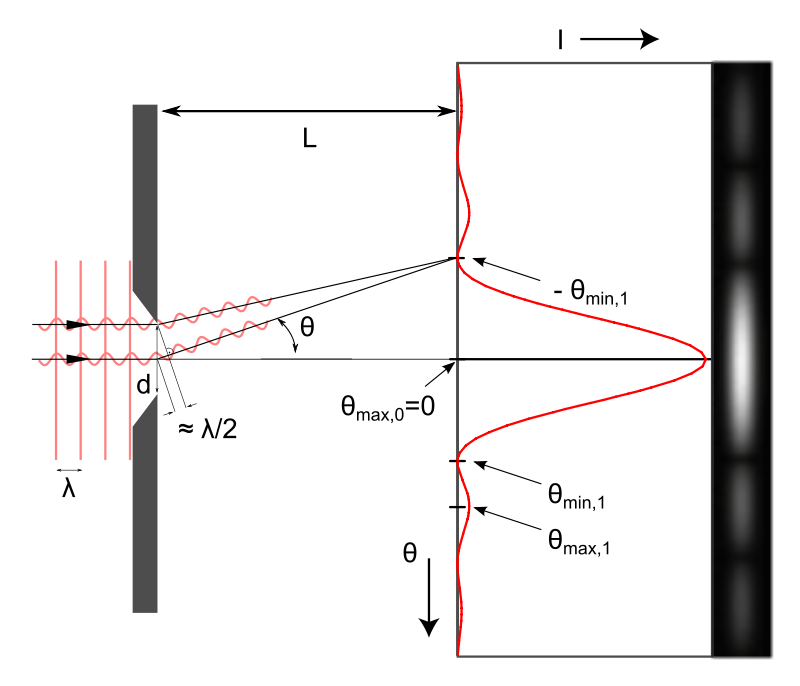
\includegraphics[width=0.6\linewidth]{generalIssues/Figures/diffraction.png}
	\end{subfigure}
	\caption{Dyfrakcja na pojedynczej szczelinie.}
	\label{diffracion}
\end{figure}

Pierwszą najprostszą formę eksperymentu przejścia światła przez podwójną szczelinę (rysunek~\ref{diffracion2}), zwaną obecnie doświadczenie Younga wykonał Thomas Young w 1801 roku. Eksperyment ten był zaczątkiem do uznania w XIX w falowej teorii światła. 

\begin{figure} [H]
	\centering
	\begin{subfigure}{.99\textwidth}
		\centering
		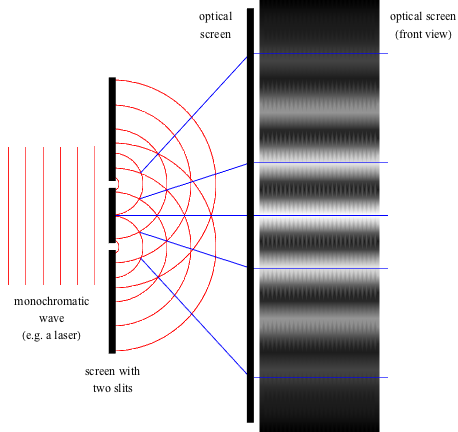
\includegraphics[width=0.6\linewidth]{generalIssues/Figures/diffraction2.png}
	\end{subfigure}
	\caption{Przejście światła przez podwójną szczelinę.}
	\label{diffracion2}
\end{figure}

Dla obrazów dyfrakcyjnych powstałych po przejściu światła przez otwór kołowy definiuje się \underline{warunek Rayleigha} określający zdolność rozdzielczą elementów i układów optycznych:\newline
$ \phi \approx \sin(\phi) = 1.22 \frac{\lambda}{d} $ (przybliżenie dla małych kątów), gdzie:\newline
$ \phi $ - minimalny kąt między promieniami, których obrazy mają być rozróżnialne, czyli inaczej – ich odległość kątowa,\newline
$ \lambda $ - długość fali światła,\newline
$ d $ - średnica otworu.\newline

Aby wzmocnić falę przechodzącą przez szczelinę stosuje się w optyce układy wielu takich szczelin, nazywane \underline{siatką dyfrakcyjną} (rysunek~\ref{diffracion3}). Efekty optyczne od każdej szczeliny dodają się, przez co zachowanie fali zależy tylko od stałej siatki (odległości dzielącej najbliższe sobie rysy). Zjawisko dyfrakcji zachodzi również, kiedy fale przechodzą przez wiele blisko siebie położonych warstw. Jeżeli odległość między warstwami jest stała, kolejne maksima fali można opisać zależnością:\newline
$ \sin(\theta) = \frac{n\lambda}{d} $, gdzie:\newline
$ d $ - stała siatki,\newline
$ \theta $ - kąt od osi wiązki światła,\newline
$ \lambda $ - długość fali,\newline
$ d $ - przyjmuje wartości całkowite dodatnie od 1,2,3,...\newline

\begin{figure} [H]
	\centering
	\begin{subfigure}{.99\textwidth}
		\centering
		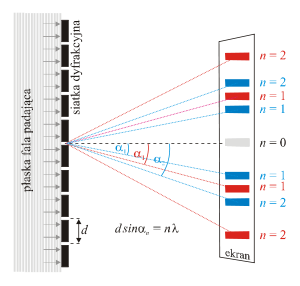
\includegraphics[width=0.6\linewidth]{generalIssues/Figures/diffraction3.png}
	\end{subfigure}
	\caption{Siatka dyfrakcyjna.}
	\label{diffracion3}
\end{figure}

Zjawisko dyfrakcji pozwoliło na rozwój krystalografii rentgenowskiej, dzięki której badano strukturę kryształów, odkryto w ten sposób także strukturę spirali DNA. 
	
	\subsection{Zasady termodynamiki.}
	\underline{Zerowa zasada termodynamiki} - jeśli układy A i B mogące ze sobą wymieniać ciepło si ą ze sobą w równowadze termicznej, i to samo jest prawdą dla układów B i C, to układy A i C również są ze sobą w równowadze termicznej. Z zasady tej wynika istnienie temperatury empirycznej. Temperatura to taka wielkość fizyczna, która dla układów A, B i C jest równa, gdy ustaje przepływ ciepła. Układy będą ze sobą w równowadze termodynamicznej. Zerowa zasada termodynamiki stwierdza także, że ciało w równowadze termodynamicznej ma wszędzie tę samą temperaturę.

\underline{Pierwsza zasada termodynamiki} - zmiana energii wewnętrznej (będącej funkcją stanu) układu zamkniętego (nie wymienia masy z otoczeniem) jest równa energii, która przepływa przez jego granice na sposób ciepła i pracy:\newline
$ \Delta U = W + Q $, gdzie:\newline
$ \Delta U $ - zmiana energii wewnętrznej układu,\newline
$ W $ - praca wykonana na układzie,\newline
$ Q $ - ciepło przekazane do układu.\newline
Alternatywne sformułowanie - nie istnieje perpetuum mobile pierwszego rodzaju (maszyna, która wytwarza więcej energii, niż sama zużywa).

\underline{Druga zasada termodynamiki} - w układzie termodynamicznie izolowanym istnieje funkcja stanu zwana entropią, która nie maleje z czasem. Matematyczny zapis tego faktu to następujące sformułowanie: zmiana entropii $ \Delta S $ w dowolnym procesie odwracalnym jest równa całce z przekazu ciepła DQ podzielonego przez temperaturę T. W procesie nieodwracalnym natomiast zmiana entropii jest większa od tej całki:
$ \Delta S \geq \int \frac{DQ}{T} $\newline
Różnica ta jest miarą nieodwracalności procesu i jest związana z rozpraszaniem energii. Entropia (S) jest funkcją stanu będąca miarą liczby sposobów (W), na jakie może być zrealizowany określony stan termodynamiczny danego układu w określonej temperaturze (T). Układ dąży do stanu, który może być w danych warunkach zrealizowany na jak najwięcej sposobów; dąży więc on do maksymalizacji entropii. Nie można bez wkładu pracy przesyłać energii termicznej między ciałami mającymi tę samą temperaturę. Oznacza to, że perpetuum mobile drugiego rodzaju (maszyna, która zamienia energię cieplną na pracę mechaniczną bez wzrostu całkowitej entropii) nie istnieje. 

\underline{Trzecia zasada termodynamiki} - nie można za pomocą skończonej liczby kroków uzyskać temperatury zera bezwzględnego (zero kelwinów), jeżeli za punkt wyjścia obierzemy niezerową temperaturę bezwzględną. Podstawą takiego zdefiniowania III zasady termodynamiki jest analiza sprawności lodówki. Jak wiemy, lodówka działa na zasadzie odwrotnego cyklu Carnota, a jej sprawność dana jest wzorem:\newline
$ n = \frac{Q_{odebrane}}{W} = \frac{T_2}{T_1-T_2} $\newline
Jeżeli ciało o określonej temperaturze $ T_1 $ chcielibyśmy schłodzić do $ T_2 \to $, odbierając przy tym skończone ciepło $ Q $, to analizując wzór widzimy, że w takim wypadku $ \frac{Q}{W} \to 0 $, czyli $ W\to $ nieskończoności. Gdybyśmy podstawili $ T_2 = 0 $, równanie nie miałoby sensu matematycznego, co oznacza, że nie da się osiągnąć temperatury zera bezwzględnego w skończonej liczbie kroków. Mówiąc inaczej, gdyby udało się schłodzić jakąś substancję do 0 K i gdyby utworzyła ona kryształ doskonały nieposiadający zamrożonych defektów krystalicznych, to jej entropia musiałaby przyjąć wartość 0. Jest to jednak technicznie, a także formalnie, niewykonalne:
$ \lim_{T\to0} S = 0 $
	
    \section{Specjalność: Eksploracja Danych i Modelowanie Interdyscyplinarne}

\end{document}
